%& /Users/ziky/.cache/org-persist/f7/163728-667e-4f03-9394-f920e669599d-832ed4017c79fd5b5d686e66a4a447c3
% Created 2025-12-08 Mon 23:59
% Intended LaTeX compiler: pdflatex
\documentclass[11pt]{article}
\usepackage[utf8]{inputenc}
\usepackage[T1]{fontenc}
\usepackage{amsmath}
\usepackage{amssymb}
\usepackage{capt-of}
\usepackage{hyperref}
\setlength{\abovedisplayskip}{0pt}
\setlength{\belowdisplayskip}{0pt}
\usepackage[a4paper, margin=1in]{geometry}

%% ox-latex features:
%   !announce-start, !guess-pollyglossia, !guess-babel, !guess-inputenc,
%   caption, maths, image, !announce-end.

\usepackage{capt-of}

\usepackage{amsmath}
\usepackage{amssymb}

\usepackage{graphicx}

%% end ox-latex features


% end precompiled preamble
\ifcsname endofdump\endcsname\endofdump\fi

\author{Ziky Zhang}
\date{\today}
\title{Worksheet \#12}
\hypersetup{
 pdfauthor={Ziky Zhang},
 pdftitle={Worksheet \#12},
 pdfkeywords={},
 pdfsubject={},
 pdfcreator={},
 pdflang={English}}
\begin{document}

\maketitle
\begin{enumerate}
\item \(1 \ \mathrm{A}\) wire of total resistance \(0.030 \ \Omega\) is bent into a triangular loop shown below, and is being pulled out of a region containing a \(2.0 \mathrm{T}\) uniform magnetic field at a speed of \(20 \ \mathrm{cm}/ \mathrm{s}\).
\begin{figure}[htbp]
\centering
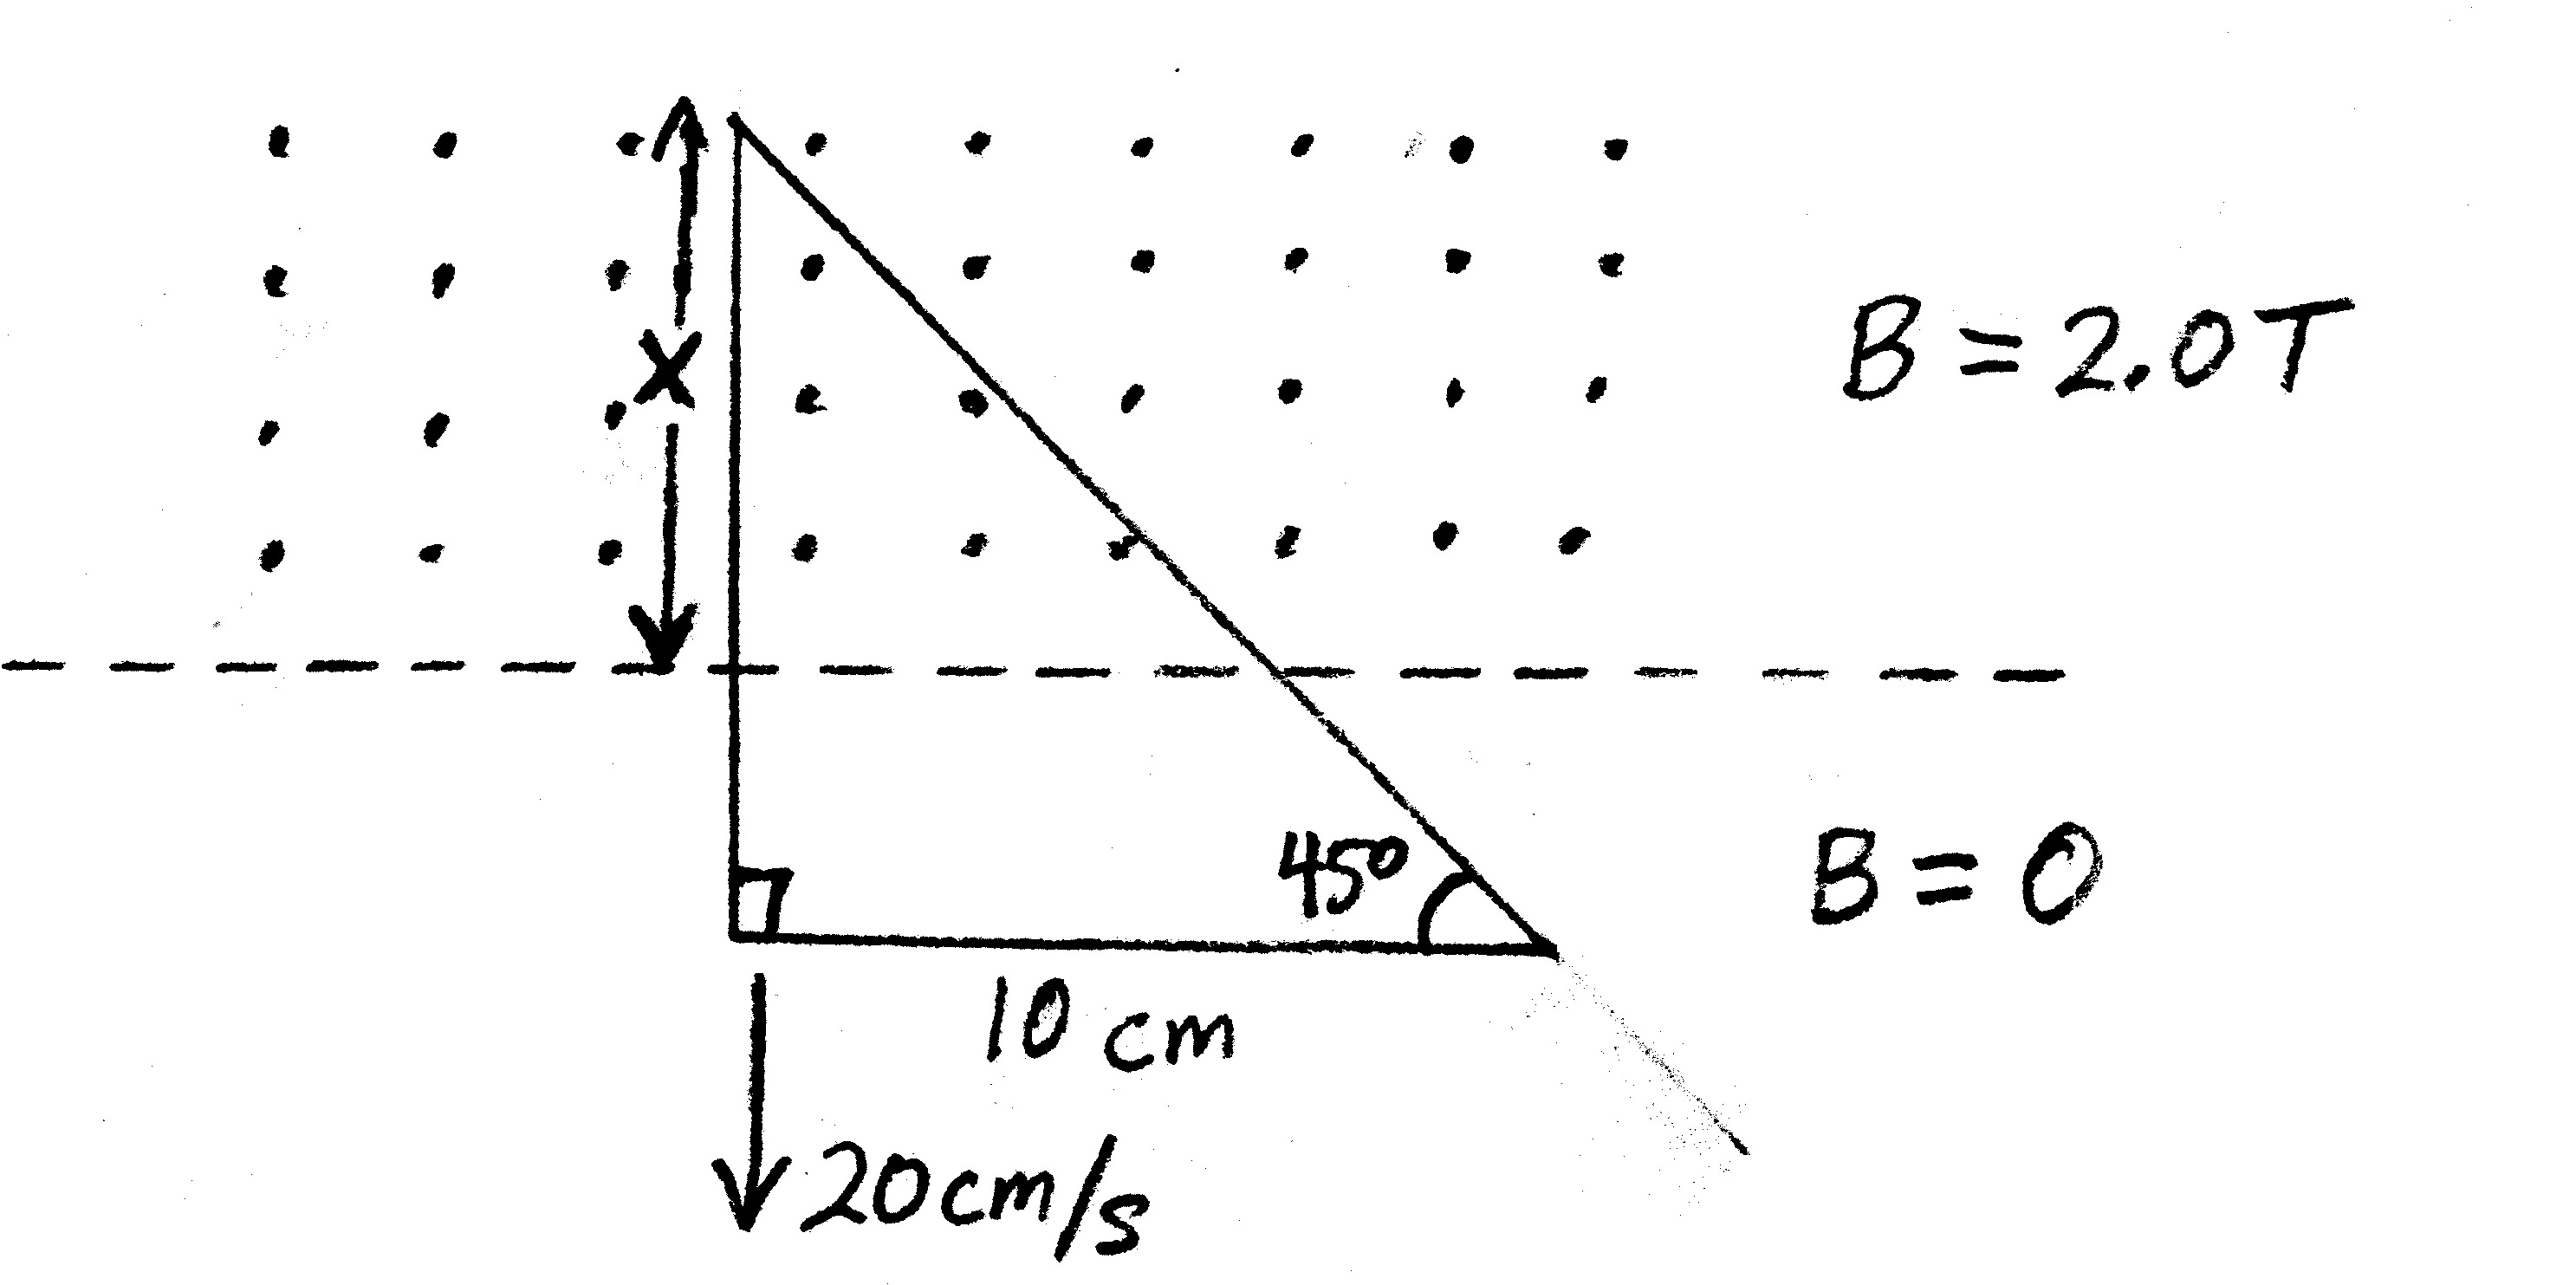
\includegraphics[height=3cm]{./img/12.1.jpg}
\caption{\label{fig:orge5c2bb0}An isosceles right triangle (leg \(10 \ \mathrm{cm}\)) leaving a magnetic field}
\end{figure}
\begin{enumerate}
\item Calculate the magnetic flux through the loop as a function of \(t\), where \(t\) is the time since the triangular loop first emerges from the field. (Hint: What is \(x(t)\)?)
\item Calculate the current in the loop at \(t = 0.20 \ \mathrm{s}\). In which direction is the current? \\
\end{enumerate}

\item A close-packed solenoid of length \(1.60 \ \mathrm{m}\) and diameter \(3.60 \ \mathrm{cm}\) has a self-inductance of \(23.0 \ \mathrm{mH}\). The solenoid is constructed from copper wiring which has a resistance of \(0.0200 \ \Omega\) for each meter of wiring. The solenoid is then connected to a \(6.00 \ \mathrm{V}\) battery which has an internal resistance of \(4.00 \ \Omega\). This is depicted below.
\begin{figure}[htbp]
\centering
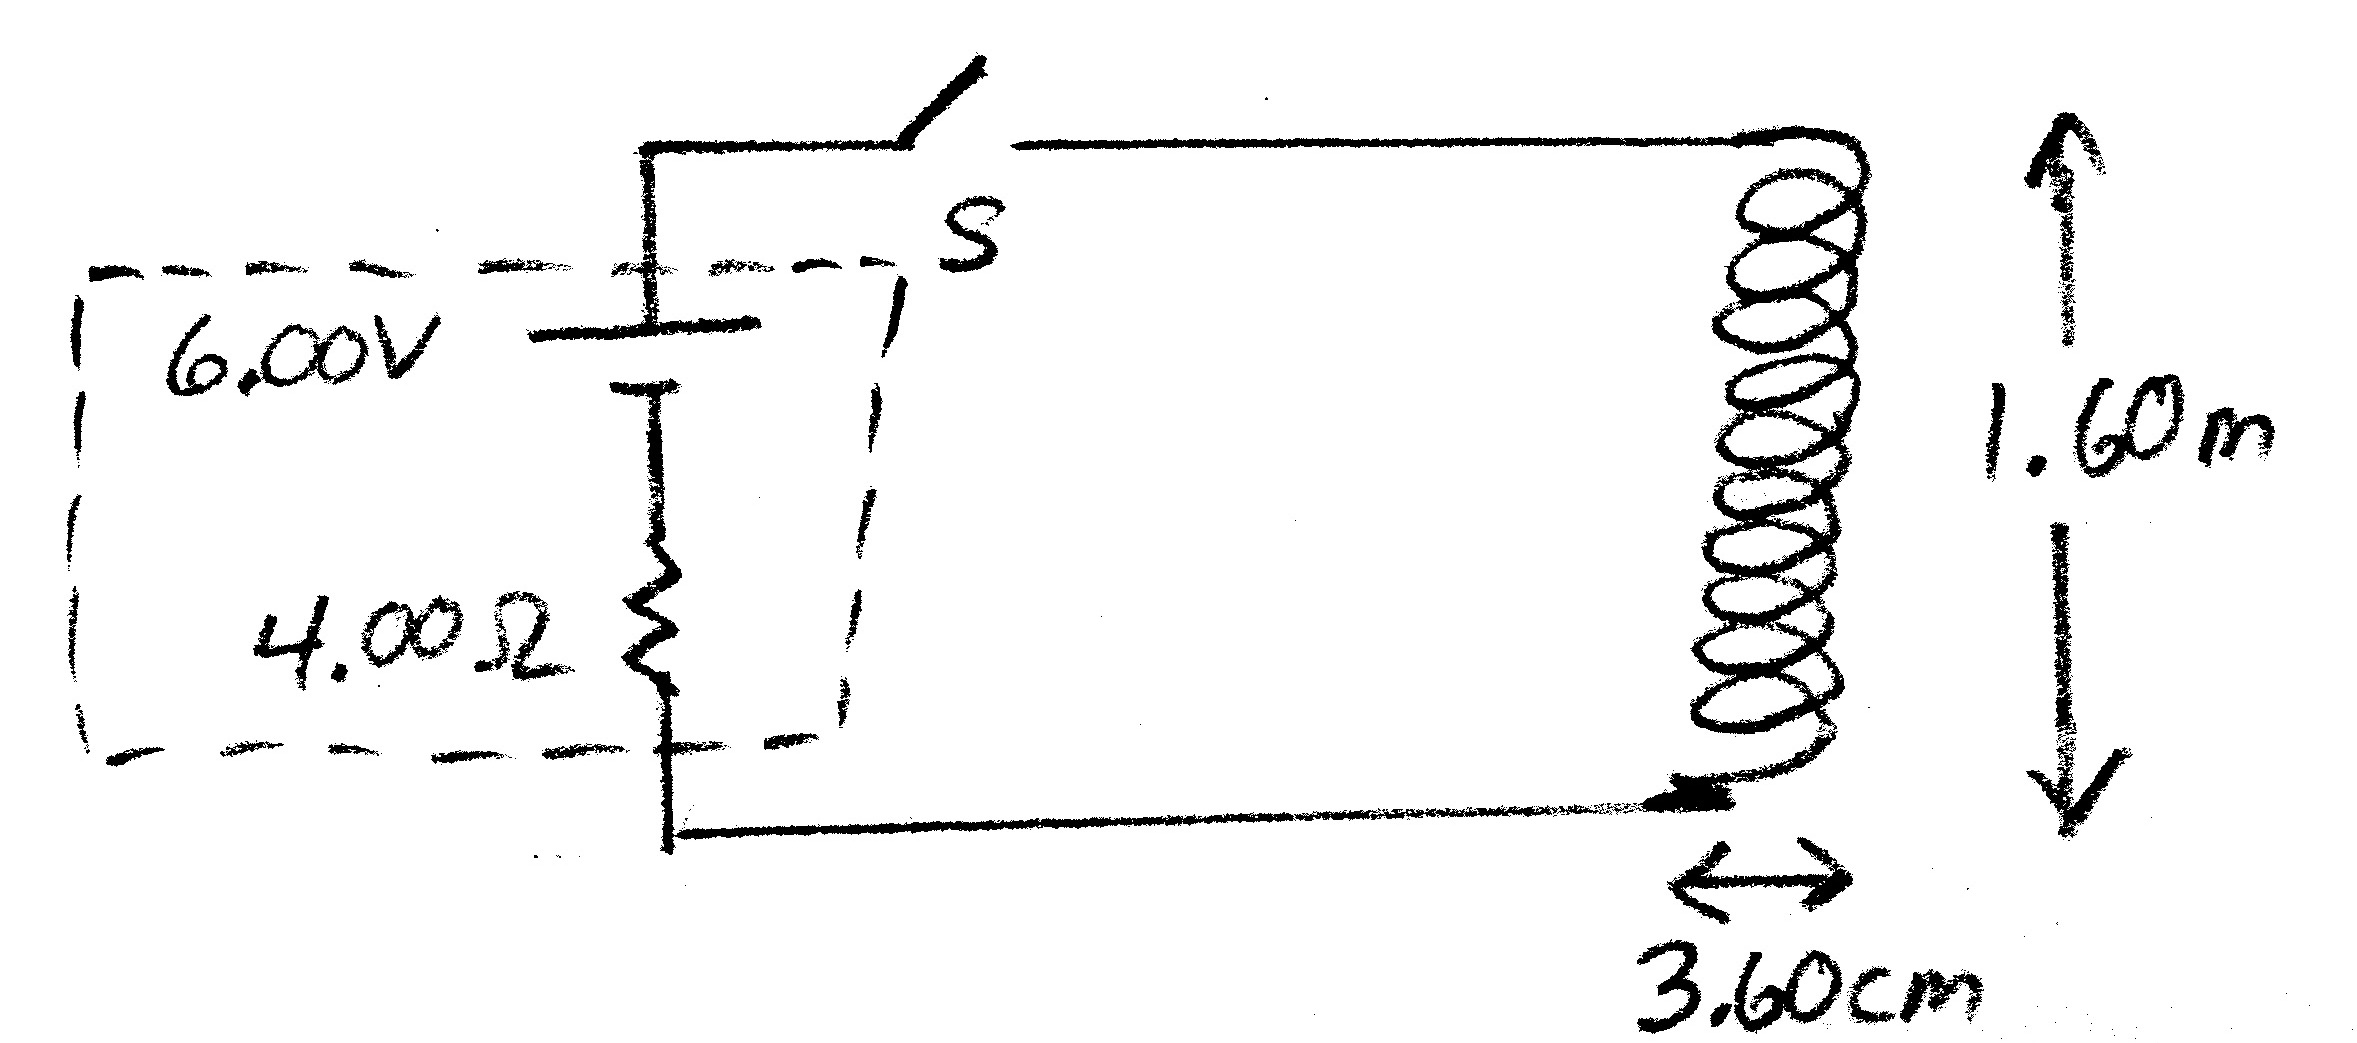
\includegraphics[height=3cm]{./img/12.2.jpg}
\caption{\label{fig:orgbb716ce}Solenoid connected to battery}
\end{figure}
\begin{enumerate}
\item Calculate the number of turns in the solenoid.
\item Calculate the time constant of the LR circuit above. Don't forget to account for the resistance of the solenoid wiring.
\item How much time is required after the switch is closed for the current in the circuit above to reach \(99.0 \%\) of its final value?
\end{enumerate}
\end{enumerate}

\newpage
\begin{align*}
\begin{aligned}[t]
\text{1.(a)} \ 
x(t) &= 0.1 - 0.2 t \ \mathrm{m} \\
a(x) &= \frac{1}{2} x^{2}\  \mathrm{m^2} \\
\Phi(t) &= \vec{B} \cdot \vec{a} \\
  &= \frac{1}{2} (0.1 - 0.2t)^2 \ \mathrm{m^2}  \cdot 2 \ \mathrm{T} \\
  &= (0.1 - 0.2t)^2 \ \mathrm{T} \mathrm{m^2} \\
\end{aligned}
\quad
\begin{aligned}[t]
\text{1.(b)} \ 
\mathcal{E}(t) &= - \frac{d\Phi}{dt} \\
  &= (- 0.01 + 0.04t - 0.04t^2) \frac{d}{dt} \\
  &= (4 - 8t) \times 10^{-2} \ \mathrm{\tfrac{Tm^2}{s}} \\ \\
I(t) &= \frac{\mathcal{E}(t)}{R} \\
  &= \frac{(4 - 8t) \times 10^{-2} \ \mathrm{\frac{Tm^2}{s}}}{3 \times 10^{-2} \ \Omega} \\
I(0.20) &= \frac{(4 - 8 \cdot 0.20 \ \mathrm{s}) \ \mathrm{\frac{Tm^2}{s}}}{3 \ \Omega} \\
  &= 0.80 \mathrm{A}
\end{aligned}
\end{align*}



\begin{align*}
\begin{aligned}[t]
\text{2.(a)} \ 
L &= \mu_0 \frac{N^2A}{l} \\
N &= \sqrt{ \frac{L \cdot l}{\mu_0 A} } \\
  &= \sqrt{ \frac{23.0 \times 10^{-3} \mathrm{H} \cdot 1.60 \ \mathrm{m}}{4\pi \times 10^{-7} \mathrm{H/m} \cdot \pi (\frac{3.6 \times 10^{-2} \ \mathrm{m}}{2})^2} } \\
  &= \sqrt{ \frac{36.8 \times 10^{-3} \mathrm{H}}{12.96 \pi^2 \times 10^{-11} \mathrm{H}} } \\
  &= \sqrt{ \frac{36.8}{12.96 \pi^2} \times 10^{8} } \\
  &= \sqrt{ 2.88 \times 10^{8} } \\
  &\approx 5366.56 \text{ turns} \\
  &\approx 5367 \text{ turns}
\end{aligned}
\quad
\begin{aligned}[t]
\text{2.(b)} \ 
\tau &= \frac{L}{R_{\mathrm{internal}} + R_{\mathrm{wiring}}} \\
  &= \frac{23.0 \times 10^{-3} \mathrm{H}}{4.00 \ \Omega + 5367 \cdot 2\pi (1.8 \times 10^{-2} \mathrm{m}) \cdot 0.0200 \ \Omega/m} \\
  &= \frac{23.0 \times 10^{-3} \mathrm{H}}{4.00 \ \Omega + 607 \ \mathrm{m} \cdot 0.0200 \ \Omega/m} \\
  &= \frac{23.0 \times 10^{-3} \mathrm{H}}{16.14 \ \Omega} \\
  &= 1.425 \times 10^{-3} \mathrm{s}
\end{aligned}
\end{align*}

2.(c)
\begin{align*}
i(t) &= i_f (1 - e^{-t/\tau_L}) \\
\frac{i(t)}{i_f} &= 1 - e^{-t/\tau_L} \\
0.99 &= 1 - e^{-t/\tau_L} \\
0.010 &= e^{-t/\tau_L} \\
- \frac{t}{\tau_{L}} &= \ln(0.010) \\
t &= - \ln(0.010) \cdot \tau_{L} \\
t &= - \ln(0.010) \cdot 1.425 \times 10^{-3} \ \mathrm{s} \\
t &= 6.56 \times 10^{-3} \ \mathrm{s}
\end{align*}
\end{document}
